\begin{frame}
    \frametitle{Material para Least Squares}
    \note{Extraído de Curso de Cyrill Stachniss https://youtu.be/r2cyMQ5NB1o?si=WYODHSkWun3FL7jR}
    \begin{itemize}
        \item Cyrill Stachniss - Least Squares - An informal Introduction \url{https://youtu.be/r2cyMQ5NB1o?si=WYODHSkWun3FL7jR}
    \end{itemize}
\end{frame}


\begin{frame}
    \frametitle{Least Squares en General}
    \note{Extraído de Curso de Cyrill Stachniss https://youtu.be/r2cyMQ5NB1o?si=WYODHSkWun3FL7jR}
    
    Enfoque para calcular una solución para un sistema sobredeterminado

    \begin{itemize}
        \item Más ecuaciones que incógnitas
        \item Minimiza la suma de cuadrados de los errores en las ecuaciones
        \item Enfoque estándar para un gran conjunto de problemas
        \item Se utiliza para estimar el modelo de parámetros dado un conjunto de observaciones
    \end{itemize}
\end{frame}

\begin{frame}
    \frametitle{Nuestro Problema}
    \note{Extraído de Curso de Cyrill Stachniss https://youtu.be/r2cyMQ5NB1o?si=WYODHSkWun3FL7jR}
    
    Dado un sistema descripto por un conjunto de $n$ funciones de observación $\left\{f_{i}\left(\state\right)\right\}_{i=1:n}$

    \begin{itemize}
        \item $\stateBold$ es el vector de estado
        \item $\observationBold$ es una una medición del estado $\stateBold$
        \item $\prediction_{i} = f_{i}\left(\stateBold\right)$ es una función que mapea el estado $\stateBold$ a una medición predicha $\prediction_{i}$
        \item Dadas $n$ mediciones ruidosas $\observationBold_{1:n}$ acerca del estado $\stateBold$
        \item Objetivo: Estimar el estado $\stateBold$ que mejor explica las mediciones $\observationBold_{1:n}$
    \end{itemize}
\end{frame}

\begin{frame}
    \frametitle{Explicación Gráfica}
    \note{Extraído de Curso de Cyrill Stachniss https://youtu.be/r2cyMQ5NB1o?si=WYODHSkWun3FL7jR}
    
    \begin{center}
        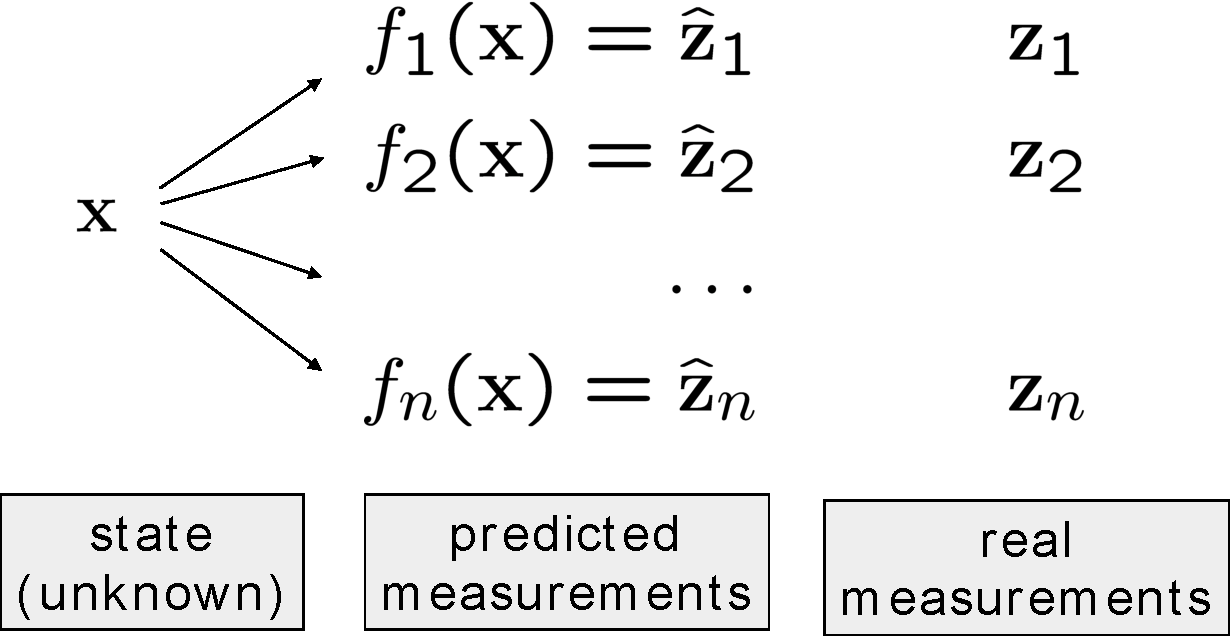
\includegraphics[width=0.7\textwidth]{images/least_squares.pdf}
    \end{center}

\end{frame}

\begin{frame}
    \frametitle{Explicación Gráfica}
    \note{Extraído de Curso de Cyrill Stachniss https://youtu.be/r2cyMQ5NB1o?si=WYODHSkWun3FL7jR}
    
    \begin{center}
        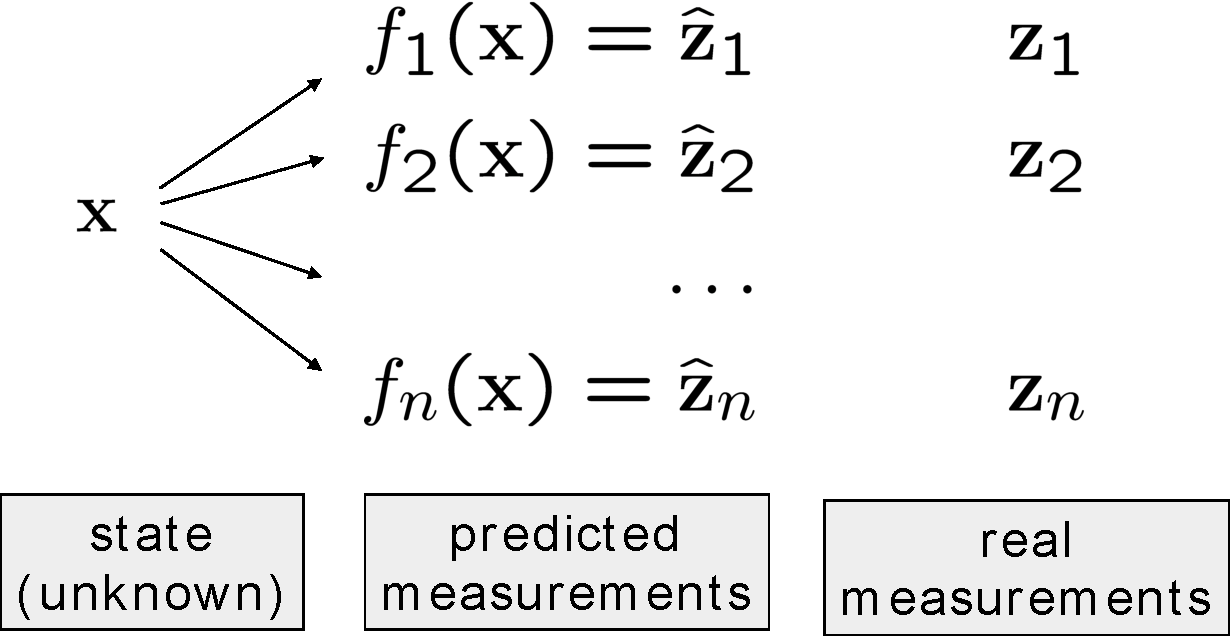
\includegraphics[width=0.7\textwidth]{images/least_squares.pdf}
    \end{center}
    
    \begin{itemize}
        \item $\stateBold$ posición de los puntos 3D
        \item $\observationBold_{i}$ coordenadas de los puntos 3D proyectados en las imágenes
        \item Estimar la posición 3D más probable de los puntos basado en las proyecciones en las imágenes (dada las poses de la cámara)
    \end{itemize}
\end{frame}

\begin{frame}
    \frametitle{Función de Error}
    \note{Extraído de Curso de Cyrill Stachniss https://youtu.be/r2cyMQ5NB1o?si=WYODHSkWun3FL7jR}
    
    \begin{itemize}
        \item $\stateBold$ posición de los puntos 3D
        \item $\observationBold_{i}$ coordenadas de los puntos 3D proyectados en las imágenes
        \item Estimar la posición 3D más probable de los puntos basado en las proyecciones en las imágenes (dada las poses de la cámara)
    \end{itemize}
\end{frame}

\begin{frame}
    \frametitle{Objetivo: Encontrar el Mínimo}
    \note{Extraído de Curso de Cyrill Stachniss https://youtu.be/r2cyMQ5NB1o?si=WYODHSkWun3FL7jR}

\end{frame}

\begin{frame}
    \frametitle{Suposiciones}
    \note{Extraído de Curso de Cyrill Stachniss https://youtu.be/r2cyMQ5NB1o?si=WYODHSkWun3FL7jR}
    
\end{frame}

\begin{frame}
    \frametitle{Solve Via Iterative Local Linearizations}
    \note{Extraído de Curso de Cyrill Stachniss https://youtu.be/r2cyMQ5NB1o?si=WYODHSkWun3FL7jR}
    
\end{frame}

\begin{frame}
    \frametitle{Linearizing the Error Function}
    \note{Extraído de Curso de Cyrill Stachniss https://youtu.be/r2cyMQ5NB1o?si=WYODHSkWun3FL7jR}
    
\end{frame}

\begin{frame}
    \frametitle{Squared Error}
    \note{Extraído de Curso de Cyrill Stachniss https://youtu.be/r2cyMQ5NB1o?si=WYODHSkWun3FL7jR}
    
\end{frame}

\begin{frame}
    \frametitle{Squared Error (cont.)}
    \note{Extraído de Curso de Cyrill Stachniss https://youtu.be/r2cyMQ5NB1o?si=WYODHSkWun3FL7jR}
    
\end{frame}

\begin{frame}
    \frametitle{Global Error}
    \note{Extraído de Curso de Cyrill Stachniss https://youtu.be/r2cyMQ5NB1o?si=WYODHSkWun3FL7jR}
    
\end{frame}

\begin{frame}
    \frametitle{Global Error (cont.)}
    \note{Extraído de Curso de Cyrill Stachniss https://youtu.be/r2cyMQ5NB1o?si=WYODHSkWun3FL7jR}
    
\end{frame}

\begin{frame}
    \frametitle{Quadratic Form}
    \note{Extraído de Curso de Cyrill Stachniss https://youtu.be/r2cyMQ5NB1o?si=WYODHSkWun3FL7jR}
    
\end{frame}

\begin{frame}
    \frametitle{Deriving a Quadratic Form}
    \note{Extraído de Curso de Cyrill Stachniss https://youtu.be/r2cyMQ5NB1o?si=WYODHSkWun3FL7jR}
    
\end{frame}

\begin{frame}
    \frametitle{Quadratic Form}
    \note{Extraído de Curso de Cyrill Stachniss https://youtu.be/r2cyMQ5NB1o?si=WYODHSkWun3FL7jR}
    
\end{frame}

\begin{frame}
    \frametitle{Minimizing the Quadratic Form}
    \note{Extraído de Curso de Cyrill Stachniss https://youtu.be/r2cyMQ5NB1o?si=WYODHSkWun3FL7jR}
    
\end{frame}

\begin{frame}
    \frametitle{Gauss-Newton Solution}
    \note{Extraído de Curso de Cyrill Stachniss https://youtu.be/r2cyMQ5NB1o?si=WYODHSkWun3FL7jR}
    
\end{frame}

\begin{frame}
    \frametitle{Example: Odometry Calibration}
    \note{Extraído de Curso de Cyrill Stachniss https://youtu.be/r2cyMQ5NB1o?si=WYODHSkWun3FL7jR}
    
\end{frame}

\begin{frame}
    \frametitle{Odometry Calibration (cont.)}
    \note{Extraído de Curso de Cyrill Stachniss https://youtu.be/r2cyMQ5NB1o?si=WYODHSkWun3FL7jR}
    
\end{frame}

\begin{frame}
    \frametitle{Questions}
    \note{Extraído de Curso de Cyrill Stachniss https://youtu.be/r2cyMQ5NB1o?si=WYODHSkWun3FL7jR}
    
\end{frame}

\begin{frame}
    \frametitle{How to Efficiently Solve the Linear System?}
    \note{Extraído de Curso de Cyrill Stachniss https://youtu.be/r2cyMQ5NB1o?si=WYODHSkWun3FL7jR}
    
\end{frame}

\begin{frame}
    \frametitle{Cholesky Decomposition for Solving a Linear System}
    \note{Extraído de Curso de Cyrill Stachniss https://youtu.be/r2cyMQ5NB1o?si=WYODHSkWun3FL7jR}
    
\end{frame}

\begin{frame}
    \frametitle{Gauss-Newton Summary}
    \note{Extraído de Curso de Cyrill Stachniss https://youtu.be/r2cyMQ5NB1o?si=WYODHSkWun3FL7jR}
    
\end{frame}

\begin{frame}
    \frametitle{Least Squares vs. Probabilistic State Estimation}
    \note{Extraído de Curso de Cyrill Stachniss https://youtu.be/r2cyMQ5NB1o?si=WYODHSkWun3FL7jR}
    
\end{frame}

\begin{frame}
    \frametitle{Start with State Estimation}
    \note{Extraído de Curso de Cyrill Stachniss https://youtu.be/r2cyMQ5NB1o?si=WYODHSkWun3FL7jR}
    
\end{frame}

\begin{frame}
    \frametitle{Log Likelihood}
    \note{Extraído de Curso de Cyrill Stachniss https://youtu.be/r2cyMQ5NB1o?si=WYODHSkWun3FL7jR}
    
\end{frame}

\begin{frame}
    \frametitle{Gaussian Assumption}
    \note{Extraído de Curso de Cyrill Stachniss https://youtu.be/r2cyMQ5NB1o?si=WYODHSkWun3FL7jR}
    
\end{frame}

\begin{frame}
    \frametitle{Log of a Gaussian}
    \note{Extraído de Curso de Cyrill Stachniss https://youtu.be/r2cyMQ5NB1o?si=WYODHSkWun3FL7jR}
    
\end{frame}

\begin{frame}
    \frametitle{Error Function as Exponent}
    \note{Extraído de Curso de Cyrill Stachniss https://youtu.be/r2cyMQ5NB1o?si=WYODHSkWun3FL7jR}
    
\end{frame}

\begin{frame}
    \frametitle{Log Likelihood with Error Terms}
    \note{Extraído de Curso de Cyrill Stachniss https://youtu.be/r2cyMQ5NB1o?si=WYODHSkWun3FL7jR}
    
\end{frame}

\begin{frame}
    \frametitle{Maximizing the Log Likelihood}
    \note{Extraído de Curso de Cyrill Stachniss https://youtu.be/r2cyMQ5NB1o?si=WYODHSkWun3FL7jR}
    
\end{frame}

\begin{frame}
    \frametitle{Minimizing the Squared Error is Equivalent to Maximizing the Log Likelihood of Independent Gaussian Distributions}
    \note{Extraído de Curso de Cyrill Stachniss https://youtu.be/r2cyMQ5NB1o?si=WYODHSkWun3FL7jR}
    
\end{frame}

\begin{frame}
    \frametitle{Summary}
    \note{Extraído de Curso de Cyrill Stachniss https://youtu.be/r2cyMQ5NB1o?si=WYODHSkWun3FL7jR}
    
\end{frame}

\begin{frame}
    \frametitle{Literature}
    \note{Extraído de Curso de Cyrill Stachniss https://youtu.be/r2cyMQ5NB1o?si=WYODHSkWun3FL7jR}
    
\end{frame}